\section{Introduction}\label{sec:introduction}
\begin{figure*}[t!]
    \centering
    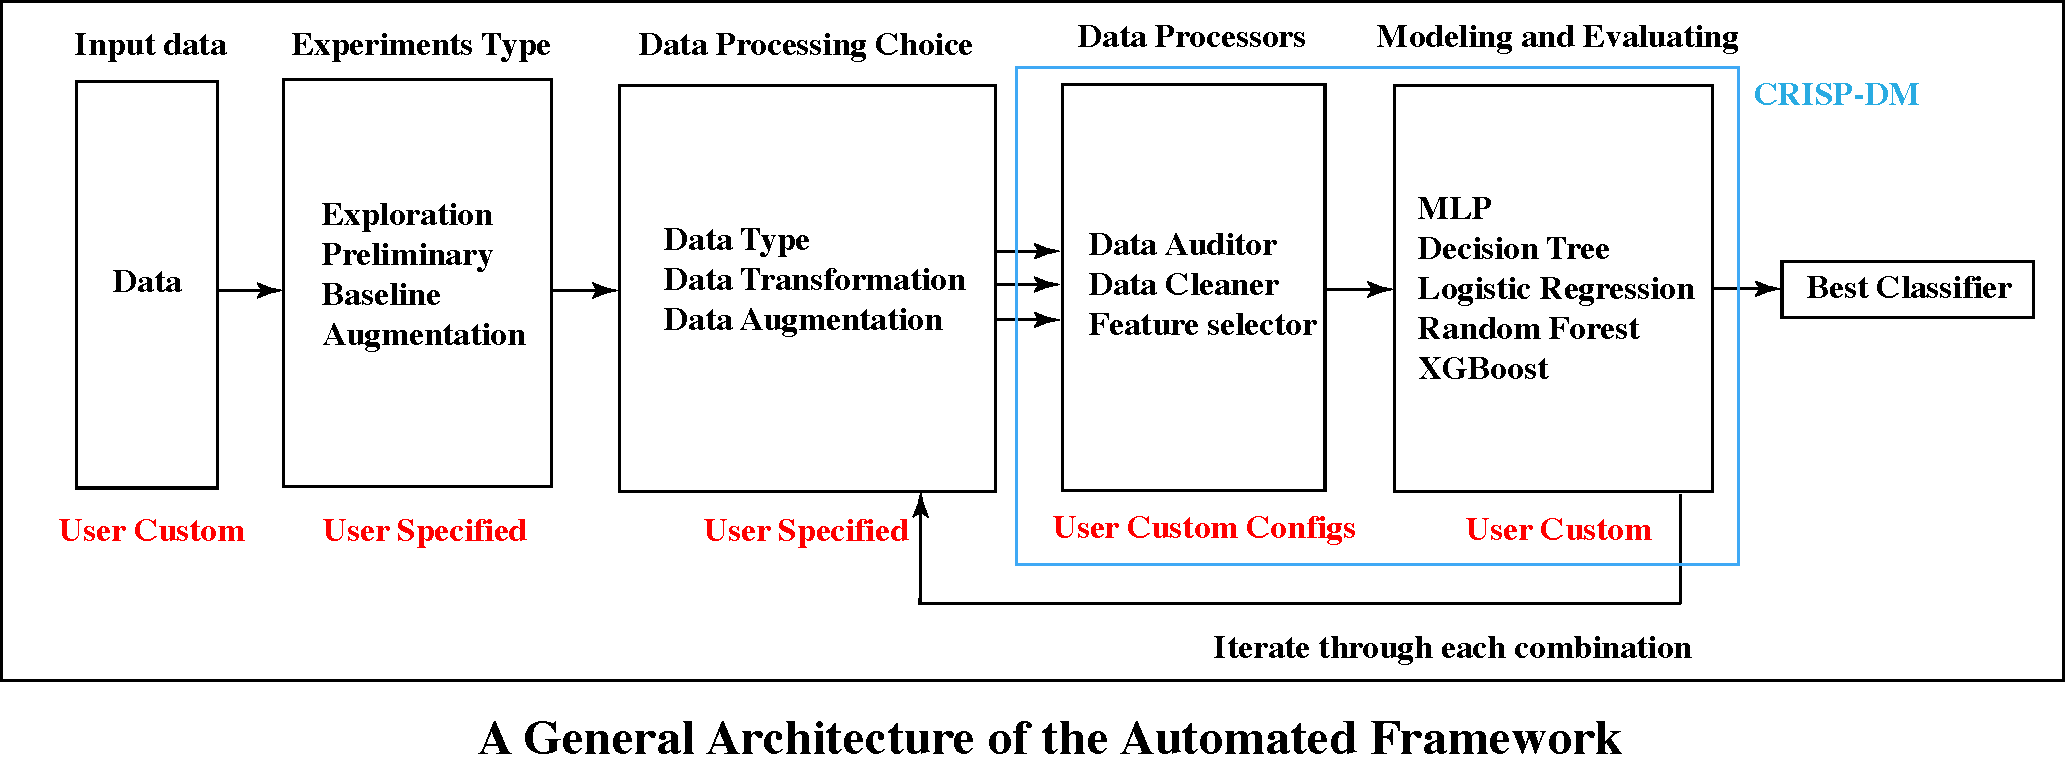
\includegraphics[width=\linewidth]{Figures/Figure1.pdf}
    \caption{A general architecture of the automated framework. The main steps for using this framework contain the following steps: 1. choose the dataset to use, 2. choose the type of benchmarking experiments to run, 3. specify which combination of data processing choice to use, 4. iterate through CRISP-DM process for each combination of data processing choice to explore the best classifier.}
    \label{fig:figure1}
\end{figure*} 

Identifying cooperative survey respondents is an important task since many surveys risk processing falsified data by taking untruthful responses seriously. This is particularly true for interviews taking place over technology where respondents may not feel as accountable for their responses. In our study we explored how to build a good performing classifier to classify the cooperativeness of the respondents, where its performance is aimed to be improved by data augmentation and transformation methods. To classify the cooperativeness, specific to our dataset ``The Attack on America and Civil Liberties Trade-Offs: A Three-Wave National Panel Survey, 2001-2004'' ~\cite{data}, we used a feature that tracks cooperativeness to be an indicator of the quality of the responses. When a respondent has a high cooperation level, we assume that data is of high quality and should be processed. 

Throughout our experiments, we faced three major challenges. Our dataset contained noisy, imbalanced, and biased data. To address the noisiness of our dataset we developed a series of data processing pipelines to reduce noise which we describe in Data Processing section of Data and Methods. To address the class imbalances, we employed a variety of data augmentation methods which we have compared the effectiveness of in our results section. To reduce the batch effects also referred to as data bias, we removed the variables causing the batch effect and proposed a data transformation method to reformat the dataset in a denser representation better fit for machine learning classifiers. 

Our study makes contributions to benchmarking data augmentation methods, generating high fidelity data, and mitigating batch effects of the data. We designed and implemented a user-friendly and automatic framework to benchmark data augmentation methods, with a reproducible data processing pipeline to create data. Using data augmentation methods to generate high fidelity training data, we created a classifier that predicts respondents’ cooperativeness during the interview with high performance. We also proposed a data transformation method to mitigate the batch effect, or form of data bias, found in our dataset. 
\begin{table}[!t]
\caption{Table of size of training data with and without data augmentation methods. The size of testing data (684, 226) is the same regardless of the methods. The size is doubled when the sample-based methods are augmented with GAN.}
\label{tab:table1}
\scalebox{0.68}{
\begin{tabular}{lcccccc}
\toprule
              & Baseline & SMOTE & editENN  & TomekLinks & SMOTEENN & SMOTETomek \\ \hline
Untransformed & 1044(684)       & 2184  & 1044 & 1044       & 1058     & 2082       \\
Transformed   & 360(226)        & 638   & 192  & 360        & 166      & 552        \\ \bottomrule
\end{tabular}
}
\end{table}